\documentclass[11pt]{beamer}
\usetheme{Berlin}
\usepackage[utf8]{inputenc}
\usepackage[spanish]{babel}
\spanishdecimal{.}
\usepackage{amsmath}
\usepackage{amsfonts}
\usepackage{amssymb}
\usepackage{color}
\usepackage{booktabs}
\usepackage{listings}
\usepackage{enumerate} 
\usecolortheme{Dolphin}
\usepackage{graphicx}
\graphicspath{{Geo/}}
\usepackage{epstopdf}
\usepackage{subfigure}
\author{Equipo A}
\date{4 de noviembre del 2020}
\title{Variables uniformes discretas}
\institute{Universidad Autónoma de Yucatan}
%\logo{
\includegraphics[width=2.0cm]{fig/Univ}}
\titlegraphic{
\includegraphics[width=2.0cm]{fig/Univ}}
%\setbeamercovered{transparent} 
%\setbeamertemplate{navigation symbols}{} 
%\logo{} 
%\institute{} 
%\date{} 
%\subject{} 
\begin{document}

\begin{frame}
\titlepage
\end{frame}

%\begin{frame}
%\tableofcontents
%\end{frame}
\begin{frame}{Competencia de la unidad}
\begin{center}
Calcula probabilidades relacionadas con las distribuciones más comunes como la Exponencial, Normal, la t
de Student, Chi-Cuadrada, F de Fisher, Binomial y Poisson, de manera adecuada.
\end{center}
\end{frame}
\begin{frame}{Actividades que realizaremos}
\begin{enumerate}
\item Resultado de aprendizajes
\item Experimento que origina a la variable uniforme discreta.
\item Deducir la función masa de probabilidad de la variable uniforme discreta.
\item Calcular la esperanza matemática de la variable uniforme discreta.
\item Calcular la varianza de la variable variable uniforme discreta.
\item Ejercicios resuelto con la función masa de probabilidad de la variable uniforme discreta.
\end{enumerate}
\end{frame}

\begin{frame}{Tema: Variables uniformes discretas}
\begin{center}
\textbf{Resultados de aprendizaje:}\\
Resuelve problemas que involucran el cálculo de probabilidades, utilizando la variable aleatoria discreta adecuada
\end{center}
\end{frame}

\begin{frame}{Experimento que origina a la variable uniforme discreta}
Es la distribución de probabilidad se asocia a variables cuyos posibles valores tienen todos la misma probabilidad. Si una variable aleatoria X cuyos posibles valores son $({x_{1}, . . . ,x_{n}})$  
tiene distribución uniforme discreta entonces
$$
P(X=x_{1})=P(X=x_{2})=...=P(X=x_{n})={\dfrac{1}{n}}
$$
\end{frame} 

\begin{frame}{Experimento que origina a la variable uniforme discreta II}
Decimos que una variable aleatoria X tiene una distribución uniforme discreta sobre el conjunto de n números $\lbrace x_{1},...,x_{n} \rbrace$ si la probabilidad de que X tome cualquiera de estos valores es constante $\dfrac{1}{n}$ . \\
Esta distribucion surge en espacios de probabilidad equiprobables, esto es, en situaciones en donde tenemos n resultados diferentes y todos ellos tienen la misma probabilidad de ocurrir. 

Los juegos de lotería son un ejemplo donde puede aplicarse esta distribucion de probabilidad. 
\end{frame}

\begin{frame}{Experimento que origina a la variable uniforme discreta III}
Se escribe:
$$X \sim unif(x_{1},...,x_{n})$$
En donde el simbolo $"\sim"$ se lee “se distribuye como” o “tiene una distribución”. La función de probabilidad de esta variable aleatoria es.
\end{frame}

\begin{frame}{Función masa de probabilidad de la variable uniforme discreta}
La función masa de probabilidad de esta variable aleatoria es:
$$
f_{X} (x)=\begin{cases}
\ {\dfrac{1}{n}} & si \mbox{ $x=x_{1},...,x_{n}$}\\{0 }& \mbox{otro caso}\
\end{cases}
$$
\end{frame}
\begin{frame}{Función masa de probabilidad de la variable uniforme discreta II}
\textbf{Ejemplo}
La gráfica de la función de probabilidad de la distribución
uniforme en el conjunto (1,2,3,4,5) aparece en la figura siguiente, junto con la correspondiente función de distribución. Cada salto en la función de distribución es de tamaño $\dfrac{1}{5}$. La expresión completa de F(x) es la siguiente:
\end{frame}
\begin{frame}{Función masa de probabilidad de la variable uniforme discreta III}
$$
F_{X} (x)=\begin{cases}
\ {0} &  \mbox{ $x<1$}\\ {0.20} &  \mbox{ $1\leq x<2$}\\ {0.40} &  \mbox{ $2\leq x<3$}\\ {0.60} &  \mbox{ $3\leq x<4$}\\ {0.80} &  \mbox{ $4\leq x<5$}\\ {1} &  \mbox{$ x\geq 5$}\
\end{cases}
$$
\end{frame}

\begin{frame}{Gráfica de la función masa de probabilidad}
\begin{center}
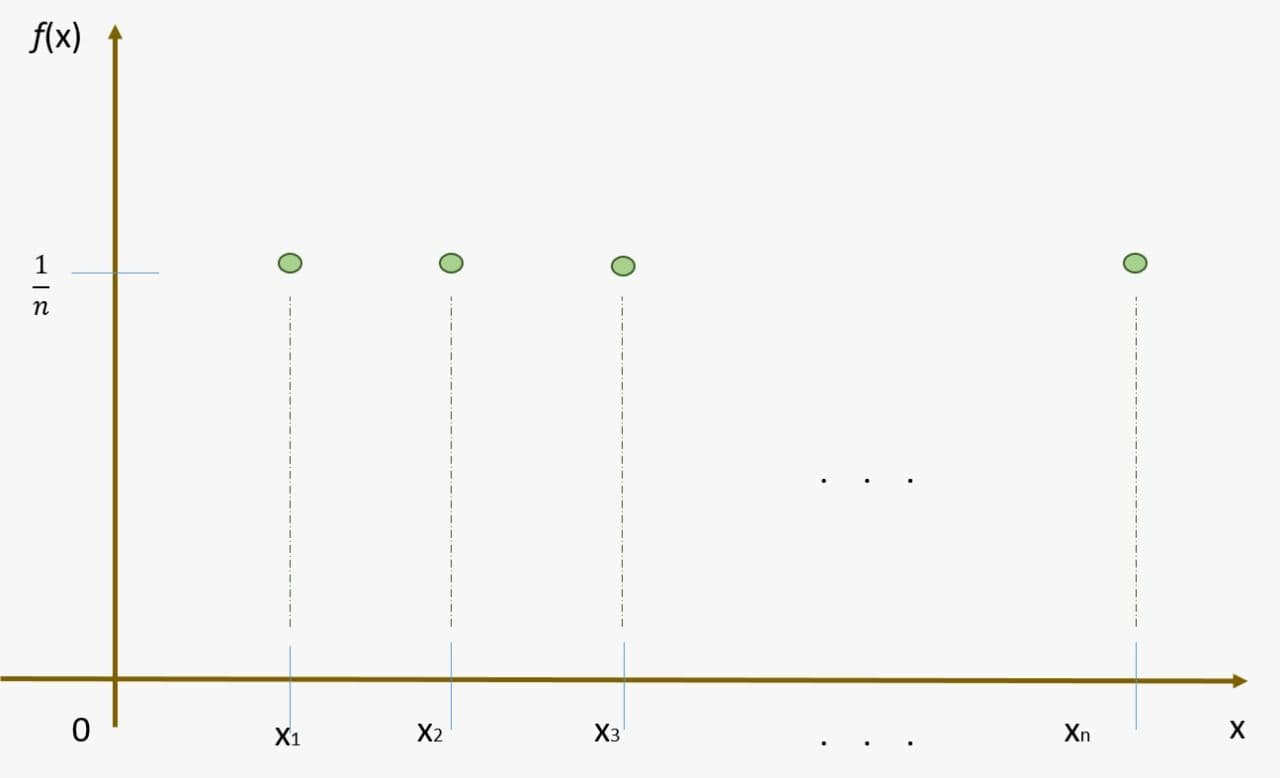
\includegraphics[scale=0.3]{grafica2.jpg}
\end{center}
\end{frame}

\begin{frame}{Gráfica de la función de distribución}
\begin{center}
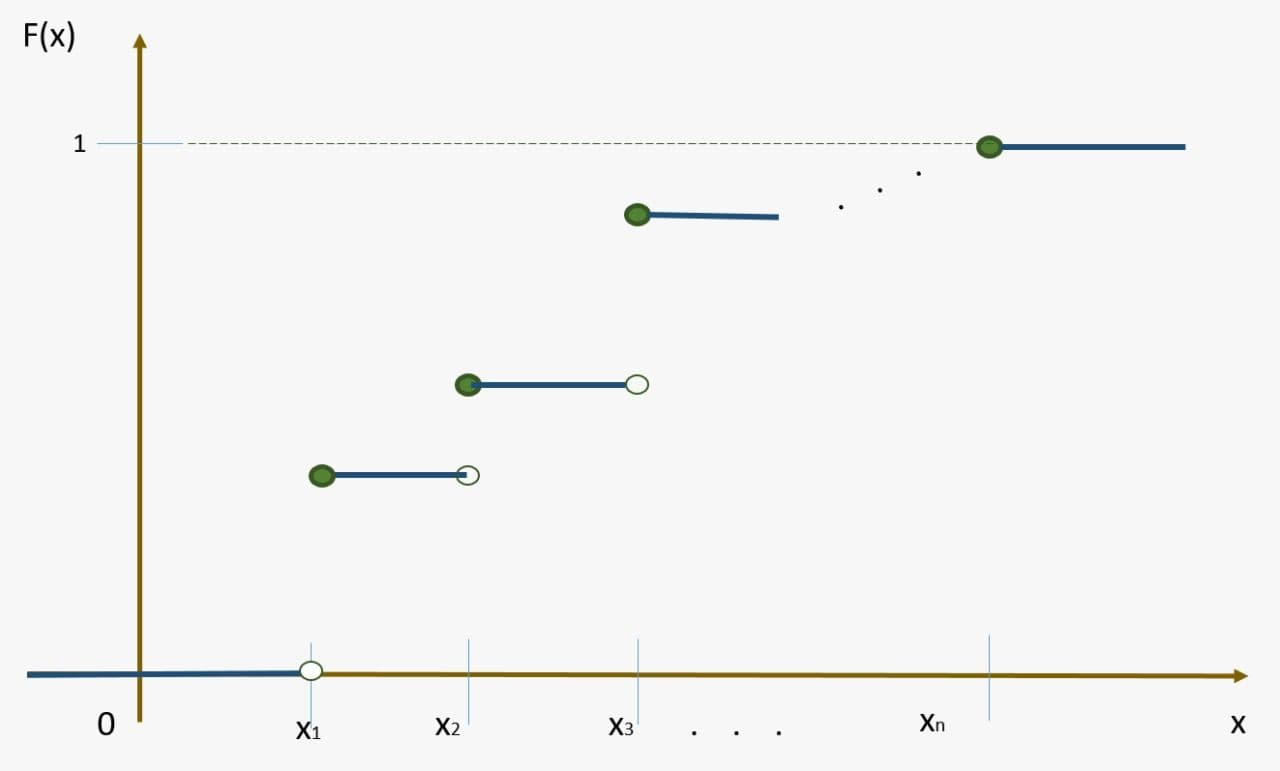
\includegraphics[scale=0.3]{grafica1.jpg}
\end{center}
\end{frame}

\begin{frame}{Calcular la esperanza matemática}
La esperanza de esta distribución puede ser obtenida como una media aritmética de los valores que toma la variable $\lbrace  x_{1},x_{2},...,x_{n} \rbrace$ y es denotada por E(X).
$$E(X)=\sum_{i=1}^{n}x_{i}f_X(x_{i})=\dfrac{1}{n}\sum_{i=1}^{n}x_{i}=\mu$$. 
\end{frame}

\begin{frame}{Propiedades de la esperanza matemática}
De la misma manera si X es una variable aleatoria  con distribución uniforme discreta en el conjunto $\lbrace 1,...,n \rbrace$. La esperanza cuenta con las siguientes propiedades:
\begin{block}{Propiedades}
a) $E(X) = \dfrac{n + 1}{2}$ \\
b) $E(X^2) = \dfrac{(n + 1)(2n + 1)}{6}$
\end{block}
\end{frame}

\begin{frame}{Demostración de la propiedad a)}
Sabemos que:
$$E(x)=\dfrac{1}{n}\sum_{i=1}^{n}x_{i}$$
Conocemos por información previa que la sumatoria de $\lbrace 1,...,n \rbrace$ puede ser vista como $\dfrac{n(n+1)}{2}$. \\
Así que: 
$$E(X)= \dfrac{1}{n}\sum_{i=1}^{n}x_{i} = \dfrac{1}{n} \cdot \dfrac{n(n+1)}{2} = \dfrac{n + 1}{2}$$
\end{frame}

\begin{frame}{Demostración de la propiedad b)}
Sabemos que:
$$E(x)=\dfrac{1}{n}\sum_{i=1}^{n}x_{i}$$
Conocemos por información previa que la sumatoria de los cuadrados de $\lbrace 1,...,n \rbrace$ puede ser vista como $\dfrac{n(n+1)(2n+1)}{6}$.\\
Así que:
$$E(X^2)= \dfrac{1}{n}\sum_{i=1}^{n}x^2_{i} = \dfrac{1}{n} \cdot \dfrac{n(n+1)(2n+1)}{6}  = \dfrac{(n + 1)(2n + 1)}{6}$$
\end{frame}

\begin{frame}{Calcular la varianza}
La varianza se obtiene de la forma ya conocida; es decir, como la varianza de esos mismos valores. Expresada en términos de momentos, la varianza será:
$$Var(X)=\dfrac{1}{n}\sum_{i=1}^{n}(x_{i}-\mu)^{2}= \dfrac{1}{n}\sum_{i=1}^{n}(x_{i})^2 - (\mu)^{2} =\sigma ^{2}$$
\end{frame} 

\begin{frame}\frametitle{Propiedades de la varianza}
De igual forma si X es una variable aleatoria  con distribución uniforme discreta en el conjunto $\lbrace 1,...,n \rbrace$. La varianza se puede resumir a:
\begin{block}{Propiedad}
$$Var(X) = \dfrac{n^{2} + 1}{12}$$
\end{block}
\end{frame}

\begin{frame}{Demostración}
Sabemos que:
$$Var(X)= \dfrac{1}{n}\sum_{i=1}^{n}(x_{i})^2 -(\mu)^{2}$$
Recordando un poco de la ley distributiva de la sumatoria, esto se podría ver cómo:
$$Var(X) =  \dfrac{1}{n}\sum_{i=1}^{n}(x_{i})^2 - \dfrac{1}{n}\sum_{i=1}^{n}(\mu)^{2}$$
Y estose puede ver de la siguiente manera:
$$Var(X) =E(X^2) - E^2(X)$$
\end{frame}

\begin{frame}{Continuación de la demostración}
Por demostraciones anteriores que realizamos en subtemas atrás, sabemos que:
$$Var(X) = E(X^2) - E^2(X)= \dfrac{(n + 1)(2n + 1)}{6} - \dfrac{(n +1)^2}{4}$$
$$=\dfrac{8n^2 + 12n + 1 - 6n^2 - 12n - 6}{24}$$
$$= \dfrac{2n^2 - 2}{24}$$
$$= \dfrac{n^2 - 1}{12}$$
\end{frame}

\begin{frame}{Ejercicios}
\begin{block}{Ejercicio 1}
Supongamos que se lanza una vez un dado. Si el dado está equilibrado:

a) Defina la funcion masa de probabilidad.\\
b) Calcule la esperanza.\\
c) Calcula la varianza.
\end{block}
\end{frame}

\begin{frame}{Solución de a)}
Observemos que X es discreta pues $R_{X}=\lbrace 1, 2, 3, 4, 5, 6 \rbrace$. Luego las posibilidades son:
$$f_{X}(1)=P(x=1)=\dfrac{1}{6}$$
$$f_{X}(2)=P(x=2)=\dfrac{1}{6}$$$$f_{X}(3)=P(x=3)=\dfrac{1}{6}$$
$$f_{X}(4)=P(x=4)=\dfrac{1}{6}$$
$$f_{X}(5)=P(x=5)=\dfrac{1}{6}$$
$$f_{X}(6)=P(x=6)=\dfrac{1}{6}$$
\end{frame}

\begin{frame} {Solución de a) II}
En conclusion:
$$
f_{X} (x)=\begin{cases}
{\dfrac{1}{6}} & si \mbox{ $x= 1,2 ,3, 4, 5, 6$}\\{0 }& \mbox{otro caso}\
\end{cases}
$$
\end{frame}

\begin{frame}{Solución de b)}
Como la variable aleatoria X tiene distribucion uniforme discrte, por deficion tenemos que:

        $$E(x)=\dfrac{1}{n}\sum_{i=1}^{n}x_{i}$$
        $$=\dfrac{1}{6}\sum_{i=1}^{6}x_{i}=\dfrac{1}{6}(1+2+3+4+5+6)$$
        $$=3.5$$
(\textbf{Nota:} Igual se pudo realizar con las propiedades de la esperanza matemática y nos daría el mismo resultado.)
\end{frame}
\begin{frame}{Solución de c)}
Como la variable aleatoria X tiene distribucion uniforme discreta, por deficion tenemos que:

        $$Var(x)=\dfrac{1}{n}\sum_{i=1}^{n}(x_{i}-\mu)^{2}$$
        $$=\dfrac{1}{6}\sum_{i=1}^{6}(x_{i}-3.5)^{2}$$
        $$=\dfrac{35}{12}$$
(\textbf{Nota:} Igual se pudo realizar con la propiedad de la varianza y nos daría el mismo resultado.)
\end{frame} 

\begin{frame}{Ejercicio 2}
En la fabricación de un cierto producto se produce con fallas, suponiendo que el numero de fallas sigue la siguiente distribucion uniforme:
$$
f_{X} (x)=\begin{cases}
\ {\dfrac{1}{5}} &\mbox{ $x=1,2,3,4,5$}\\ {0} &\mbox{otro caso}\
\end{cases}
$$
Determine la probabilidad de que en cierto producto se encuentren: 

a) 2 fallas.

b) 3 fallas.

c)Mas de 3 fallas.

\end{frame} 
 
\begin{frame}{Solucion a)}
Esto lo podemos ver como:

$$P(x=2)=f(2)=\frac{1}{5}$$

\end{frame} 

\begin{frame}{Solucion b)}
Esto lo podemos ver como:

$$P(x=3)=f(3)=\frac{1}{5}$$


\end{frame} 

\begin{frame}{Solucion c)}
Esto lo podemos ver como:

$$P(x>3)=f(4)+f(5)+f(6)+...+f(n)=\frac{1}{5}+\frac{1}{5}+0+...+0$$
$$=\frac{2}{5}$$


\end{frame}  
 
\end{document}
